  
 
  
  
\begin{frame}\frametitle{Factors flow graph} 
  
  
\begin{center} 
  
  
\begin{figure} 
  
  
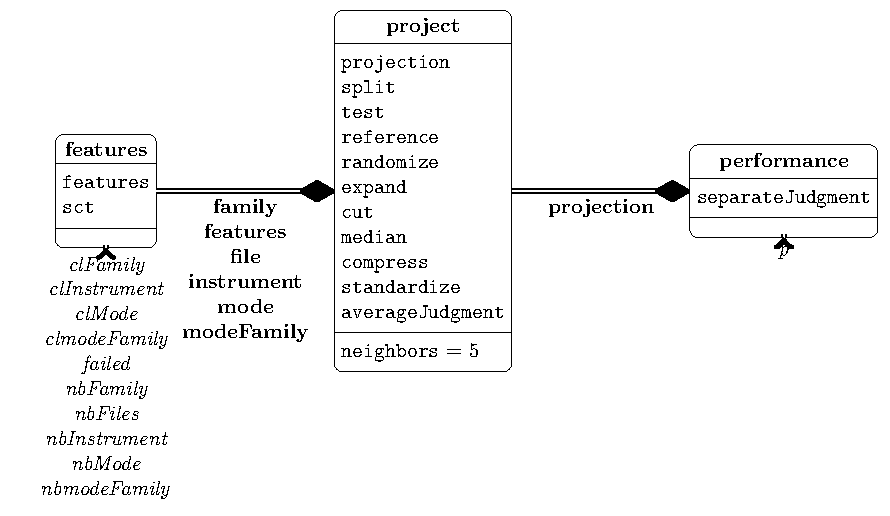
\includegraphics[width=\textwidth,height=0.8\textheight,keepaspectratio]{../figures/factors.pdf} 
  
  
\label{factorFlowGraph} 
  
  
\end{figure} 
  
  
\end{center} 
  
  
\end{frame} 
  
\begin{frame}\frametitle{sct: 25, projection: lmnn, split: none, reference: judgments, randomize: 0, expand: 0, cut: 1, median: 1, compress: 1, standardize: 1, averageJudgment: 0} 
  
\begin{table} 
\begin{center} 
\ 
 \setlength{\tabcolsep}{.16667em} 
\begin{tabular}{llc} 
fea & sepjud & p (\%) \\ 
\hline 
mfcc & 0 & 86.3 \\ 
mfcc & 1 & 86.2 \\ 
mfcc & 2 & 85.1 \\ 
scat & 0 & 91.6 \\ 
scat & 1 & 95.2 \\ 
scat & 2 & 86.4 \\ 
tfscat & 0 & \textbf{96.2} \\ 
tfscat & 1 & \textbf{\textcolor{red}{96.9}} \\ 
tfscat & 2 & 91.1 \\ 
\end{tabular} 
\end{center} 
\label{sc25PrlmSpnoRejuRa0Ex0Cu1Me1Co1St1Avju0} 
\end{table} 
 
\end{frame}  
